\documentclass[11pt, addpoints, answers]{exam}

\usepackage[utf8]{inputenc}
\usepackage[T1]{fontenc}
\usepackage[margin  = 1in]{geometry}
\usepackage{amsmath, amscd, amssymb, amsthm, verbatim}
\usepackage{mathabx}
\usepackage{setspace}
\usepackage{float}
\usepackage{color}
\usepackage{graphicx}
\usepackage[colorlinks=true]{hyperref}
\usepackage{tikz}

\usetikzlibrary{shapes,arrows}
%%%<
\usepackage{verbatim}
%%%>
\usetikzlibrary{automata,arrows,positioning,calc}

\usetikzlibrary{trees}

\shadedsolutions
\definecolor{SolutionColor}{RGB}{214,240,234}

\newcommand{\bbC}{{\mathbb C}}
\newcommand{\R}{\mathbb{R}}            % real numbers
\newcommand{\bbR}{{\mathbb R}}
\newcommand{\Z}{\mathbb{Z}}            % integers
\newcommand{\bbZ}{{\mathbb Z}}
\newcommand{\bx}{\mathbf x}            % boldface x
\newcommand{\by}{\mathbf y}            % boldface y
\newcommand{\bz}{\mathbf z}            % boldface z
\newcommand{\bn}{\mathbf n}            % boldface n
\newcommand{\br}{\mathbf r}            % boldface r
\newcommand{\bc}{\mathbf c}            % boldface c
\newcommand{\be}{\mathbf e}            % boldface e
\newcommand{\bE}{\mathbb E}            % blackboard E
\newcommand{\bP}{\mathbb P}            % blackboard P

\newcommand{\ve}{\varepsilon}          % varepsilon
\newcommand{\avg}[1]{\left< #1 \right>} % for average
%\renewcommand{\vec}[1]{\mathbf{#1}} % bold vectors
\newcommand{\grad}{\nabla }
\newcommand{\lb}{\langle }
\newcommand{\rb}{\rangle }

\def\Bin{\operatorname{Bin}}
\def\Var{\operatorname{Var}}
\def\Geom{\operatorname{Geom}}
\def\Pois{\operatorname{Pois}}
\def\Exp{\operatorname{Exp}}
\newcommand{\Ber}{\operatorname{Ber}}
\def\Unif{\operatorname{Unif}}
\def\No{\operatorname{N}}
\newcommand{\E}{\mathbb E}            % blackboard E
\def\th{\theta }            % theta shortcut
\def\V{\operatorname{Var}}
\def\Var{\operatorname{Var}}
\def\Cov{\operatorname{Cov}}
\def\Corr{\operatorname{Corr}}
\newcommand{\epsi}{\varepsilon}            % epsilon shortcut

\providecommand{\norm}[1]{\left\lVert#1\right\rVert} %norm
\providecommand{\abs}[1]{\left \lvert#1\right \rvert} %absolute value

\DeclareMathOperator{\lcm}{lcm}
\newcommand{\ds}{\displaystyle}	% displaystyle shortcut

\def\semester{2018-2019}
\def\course{Modèles Aléatoires Discrets}
\def\title{\MakeUppercase{Examen Final}}
\def\name{Pierre-O Goffard}
%\def\name{Professor Wildman}

\setlength\parindent{0pt}

\cellwidth{.35in} %sets the minimum width of the blank cells to length
\gradetablestretch{2.5}

%\bracketedpoints
%\pointsinmargin
%\pointsinrightmargin

\begin{document}


\runningheader{\course  \vspace*{.25in}}{}{\title \vspace*{.25in}}
%\runningheadrule
\runningfooter{}{Page \thepage\ of \numpages}{}

% \firstpageheader{Name:\enspace\hbox to 2.5in{\hrulefill}\\  \vspace*{2em} Section: (circle one) TR: 3-3:50 \textbar\, TR: 5-5:50 \textbar\,  TR: 6-6:50(Xu) \textbar\,  TR: 6-6:50 }{}{Perm \#: \enspace\hbox to 1.5in{\hrulefill}\\ \vspace*{2em} Score:\enspace\hbox to .6in{\hrulefill} $/$\numpoints}
\extraheadheight{.25in}

\hrulefill

\vspace*{1em}

% Heading
{\center \textsc{\Large\title}\\
	\vspace*{1em}
	\course -- \semester\\
	Pierre-O Goffard\\
}
\vspace*{1em}

\hrulefill

\vspace*{2em}

\noindent {\bf\em Instructions:} On éteint et on range son téléphone.
\begin{itemize}
	\item La calculatrice et les appareils éléctroniques ne sont pas autorisés.
	\item Vous devez justifier vos réponses de manière claire et concise.
	\item Vous devez écrire de la manière la plus lisible possible. Souligner ou encadrer votre réponse finale.

\end{itemize}

\begin{center}
	\gradetable[h]
\end{center}

\smallskip

\begin{questions}
\question Soit $(X_n)_{n\geq0}$ une chaîne de Markov d'espace d'état $\{1,2,3\}$ de matrice de transition:
\[Q=\begin{pmatrix}
0 & 1 & 0 \\
0 & 2/3 & 1/3 \\
1/2 & 1/2 & 0
\end{pmatrix}\]
	\begin{parts}
		\part[1]  Desiner le graph des transitions de $(X_n)_n\geq0$
		\begin{solution}
			 \begin{center}
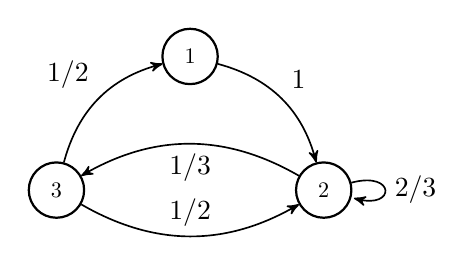
\begin{tikzpicture}[->, >=stealth', auto, semithick, node distance=3cm]
\tikzstyle{every state}=[fill=white,draw=black,thick,text=black,scale=0.8]
\node[state]    (1)                     {$1$};
\node[state]    (2)[below right of=1]   {$2$};
\node[state]    (3)[below left of=1]   {$3$};
\path
(1) edge[bend left]     node{$1$}         (2)

(2) edge[loop right]      node{$2/3$}      (2)
    edge[bend right]     node{$1/3$}      (3)
(3) edge[bend left]      node{$1/2$}      (1)
    edge[bend right]     node{$1/2$}      (2);

\end{tikzpicture}
\end{center}

		\end{solution}
		\part[1] La chaine est-elle irréductible? Combien de classe d'équivalence comprend-elle? Ces classes sont-elles ouvertes ou fermées?
		\begin{solution}
		La chaine est irréductible. Il n'y a qu'une seule classe d'équivalence qui est donc fermée.
		\end{solution}
		\part[2] Donner la loi invariante $\pi$ après voir justifier son existence et son unicité.
		\begin{solution}
		L'espace d'état est fini et la chaine de Markov est irréductible. La loi invariante existe et est unique donnée par $\pi = (1/9,6/9,2/9)$.
		\end{solution}
	\end{parts}
\question Afin de remporter la coupe d'immortalité, Harry doit vaincre trois monstres dans cet ordre
\begin{enumerate}
	\item Le Basilic (B)
	\item L'Acromentule (A)
	\item La Chimère (C)
\end{enumerate}
A chaque étape, si Harry est défait, il doit recommencer depuis le début (avec ce bon vieux basilic qui aura eu le temps de récupérer). On suppose qu'il vainc le basilic avec probabilité $0.8$, l'acromentule avec probabilité $0.6$, et la chimere avec probabilité $0.3$. S'il parvient à se défaire de la chimère alors il remporte la coupe d'immortalité (I). On utilise une chaine de Markov homogène $(X_n)_{n\geq0}$ pour suivre Harry dans sa quête.
\begin{parts}
\part[1] Donner l'espace d'état, le graph et la matrice de transition associés à la chaine de Markov $(X_n)_{n\geq0}$
\begin{solution}
L'espace d'état est $E = \{B,A,C,I\}$. Le graph des transitions est donnée par
\begin{center}
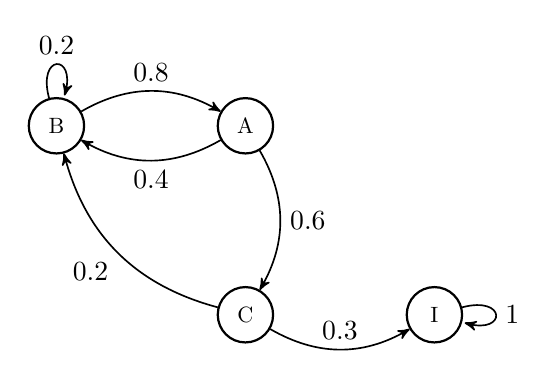
\begin{tikzpicture}[->, >=stealth', auto, semithick, node distance=3cm]
\tikzstyle{every state}=[fill=white,draw=black,thick,text=black,scale=0.8]
\node[state]    (1)                {B};
\node[state]    (2)[right of=1]    {A};
\node[state]    (3)[below of=2]    {C};
\node[state]    (4)[right of=3]    {I};
\path
(1) edge[bend left]     node{$0.8$}       (2)
    edge[loop above]    node{$0.2$}      (1)
(2) edge[bend left]     node{$0.4$}       (1)
    edge[bend left]     node{$0.6$}       (3)
(3) edge[bend left]     node{$0.2$}      (1)
    edge[bend right]    node{$0.3$}      (4)
(4) edge[loop right]     node{$1$}      (4)    ;
\end{tikzpicture}
\end{center}
La matrice de trasition est donnée par
\[Q=\begin{pmatrix}
0.2 & 0.8 & 0 & 0 \\
0.4 & 0 &0.6&0 \\
0.7 &0 & 0 & 0.3\\
0&0&0&1
\end{pmatrix}\]
\end{solution}
\part[1] Donner les classes d'équivalence, indiquer si elles sont ouvertes ou fermées.
\begin{solution}
Deux classes d'équivalence
\begin{itemize}
\item $\{B,A,C\}$ ouverte
\item $\{I\}$ fermée
\end{itemize}
\end{solution}
\part[1] Donner la période de chaque état.
\begin{solution}
Tous les états sont apériodiques (de période 1).
\end{solution}
\end{parts}
\question On suppose que le nombre de regards méchants que je reçois au cours de l'examen final est bien modélisé par un processus de Poisson d'intensité $\lambda$. L'unité de temps est l'heure et l'examen dure $2$ heures.
\begin{parts}
\part[1] Quelle est la probabilité que je reçoivent au moins $3$ regards méchants lors de la première heure? On donnera le résultat en fonction de $\lambda$.
\begin{solution}
$$
\mathbb{P}(N_1\geq 3)= 1-e^{-\lambda}\left(1+\lambda+\frac{\lambda^{2}}{2}\right)
$$
\end{solution}
\part[1] Quelle est la probabilité que je reçoivent exactement $8$ regards méchants lors de la première heure et $1$ seul regard méchant pendant les $30$ dernières minutes? On donnera le résultat en fonction de $\lambda$.
\begin{solution}
$$
\mathbb{P}(N_1=8, N_2-N_{1.5}=1)= \mathbb{P}(N_1=8)\mathbb{P}(N_2-N_{1.5}=1)=e^{-3\lambda/2}\frac{\lambda^{9}}{2\times 8!}.
$$
\end{solution}
\end{parts}
\question Une compagnie d'assurance propose un contrat d'assurance auto couvrant une année et fixe un niveau de prime en fonction du nombre d'accidents reportés l'année précédente. Pour chaque assuré, pour chaque année,
\begin{itemize}
\item Le nombre d'accident est modélisé par une variable aléatoire de comptage $N$ de loi de probabilité
\begin{equation*}
\mathbb{P}(N=0)=\frac{7}{10},\text{ }\mathbb{P}(N=1)=\frac{2}{10},\text{ et }\mathbb{P}(N=2)=\frac{1}{10}.
\end{equation*}
\item Le montant des sinistres (indemnisation que la compagnie d'assurance verse a l'assuré en cas d'accident de voiture) est une variable aléatoire positive $U$ suivant une loi hyperexponentielle $\text{HExp}(p,\delta_1,\delta_2)$ de densité
\begin{equation*}
f_U(x)=\left[p\delta_1e^{-\delta_{1}x}+(1-p)\delta_{2}e^{-\delta_{2}x}\right]\mathbb{I}_{\left[0,+\infty\right)}(x)
\end{equation*}
où $0\leq p\leq1$ et $\delta_1,\delta_2>0$.
\item Le montant agrégé des sinistres pour un assuré (La somme de toutes les indemnisations de l'année en cours) est donnée par la variable aléatoire
$$S=\sum_{k=1}^{N}U_{k},$$
où les $U_k$ sont \textbf{i.i.d.} de même loi que $U$.
\item le montant des sinistres est indépendant du nombre de sinistres ($N$ est indépendant de $U_1,U_2\ldots$). 
\end{itemize}
Les questions sont plus ou moins indépendantes.
\begin{parts}
\part[1] Calculer la moyenne de $N$, donner le résultat sous la forme d'une fraction (la plus réduite possible).
\begin{solution}
  $$
  \mathbb{E}(N)=\frac{2}{5}
  $$
\end{solution}
\part[1] Calculer la moyenne de $U$, donner le résultat sous la forme d'une fraction (la plus réduite possible) avec $p=1/2$, $\delta_1=1/4$ et $\delta_2=1/6$.
  \begin{solution}
  $$
  \mathbb{E}(U)=5
  $$
\end{solution}
\part[1] En suivant le principe de la moyenne, la prime que doit payer l'assuré est donnée par
$$
c= (1+\eta)\mathbb{E}(S).
$$
Calculer $c$ pour un chargement de sécurité $\eta = 5\%$, avec $p=1/2$, $\delta_1=1/4$ et $\delta_2=1/6$.
  \begin{solution}
  $$
  c=(1+\eta)\mathbb{E}(U)\times \mathbb{E}(N)=\frac{105}{50}=\frac{21}{10}
  $$
\end{solution}
\part[1] Calculer la variance de $S$. Donner le résultat sous la forme d'une fraction (la plus réduite possible) avec $p=1/2$, $\delta_1=1/4$ et $\delta_2=1/6$.
  \begin{solution}
  \begin{eqnarray*}
  \mathbb{V}(S)&=&\E(U)^2\V(N)+ \E(N)\V(U) \\
  &=& 25\times \frac{11}{25} + \frac{2}{5}\times 27\\
  &=& 11+\frac{54}{5}=\frac{109}{5}
  \end{eqnarray*}
\end{solution}
\part[1] On suppose maintenant que le chargement de sécurité appliqué pour un assuré évolue en fonction du nombre de sinistres reportés l'année précédente. La valeur du chargement de sécurité est dictée par une chaine de Markov homogène $(X_n)_{n\geq0}$ d'espace d'état $E=\{\eta_1,\eta_2,\eta_3\}$. On suppose que $X_0=\eta_1$, Les transitions d'un chargement de sécurité vers un autre s'effectuent de la manière suivante:
\begin{itemize}
\item L'assuré reste dans l'état $\eta_1$ si aucun accident n'est reporté, va dans l'état $\eta_2$ si un accident est reporté et va dans l'état $\eta_3$ si deux accidents de voiture sont reportés.
\item Dans l'état $\eta_2$, l'assuré va dans l'état $\eta_1$ si aucun accident de voiture n'est reporté, et va dans l'état $\eta_3$ sinon.
\item Dans l'état $\eta_3$, L'assuré va dans l'état $\eta_2$ si aucun accident de voiture n'est reporté, et reste dans l'état $\eta_3$ sinon.
\end{itemize}
Donner le graph et la matrice de transition de cette chaine de Markov.
\begin{solution}
Le graph des transitions est donné par
\begin{center}
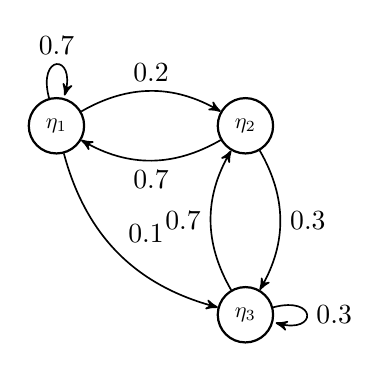
\begin{tikzpicture}[->, >=stealth', auto, semithick, node distance=3cm]
\tikzstyle{every state}=[fill=white,draw=black,thick,text=black,scale=0.8]
\node[state]    (1)                {$\eta_1$};
\node[state]    (2)[right of=1]    {$\eta_2$};
\node[state]    (3)[below of=2]    {$\eta_3$};
\path
(1) edge[bend left]     node{$0.2$}      (2)
    edge[loop above]    node{$0.7$}      (1)
    edge[bend right]     node{$0.1$}      (3)
(2) edge[bend left]     node{$0.7$}      (1)
    edge[bend left]     node{$0.3$}      (3)
(3) edge[bend left]     node{$0.7$}      (2)
    edge[loop right]    node{$0.3$}      (3);
\end{tikzpicture}
\end{center}
La matrice de transition est donnée par
\[Q=\begin{pmatrix}
0.7 & 0.2 & 0.1 \\
0.7 & 0 &0.3 \\
0 &0.7 & 0.3
\end{pmatrix}\]
\end{solution}
\part[2] Donner la loi invariante après avoir justifier son existence et son unicité.
\begin{solution}
La chaine est irréductible sur un espace d'état fini, elle admet donc une unique loi invariant donnée par
$$
\pi = (49/86\text{ }21/86 \text{ }16/86)
$$
\end{solution}
\part[2] Calculer la prime
$$
c_\infty = \mathbb{E}\left[(1+X_\infty)S\right]
$$
correspondant à la prime payée par un assuré client de la compagnie d'assurance pendant un nombre \textit{suffisant} d'années, donner le résultat en fonction de $\eta_1, \eta_2$ et $\eta_3$, avec $p=1/2$, $\delta_1=1/4$ et $\delta_2=1/6$.
\begin{solution}
\begin{eqnarray*}
c_\infty &=& \mathbb{E}\left[(1+X_\infty)\right]\mathbb{E}(S)\\
&=& \left(1+\frac{49}{86}\eta_1 +\frac{21}{86}\eta_2 +\frac{16}{86}\eta_3\right)2\\
&=& \left(2+\frac{49}{43}\eta_1 +\frac{21}{43}\eta_2 +\frac{16}{43}\eta_3\right)
\end{eqnarray*}
\end{solution}
\part[2] Supposons que la compagnie d'assurance constitue une réserve $u$ au début de chaque année et que le portefeuille contient $m$ assurés, clients de la compagnie depuis très longtemps. La probabilité de ruine, pour l'année courante, est donnée par
$$
\psi(u)=\mathbb{P}\left(u+mc_\infty-\sum_{k=1}^{m}S_k<0\right)
$$
où les $S_k$ sont des variables aléatoires \textbf{i.i.d.} distribuées comme $S$. Notons $\mu=\mathbb{E}(S)$ et $\sigma=\sqrt{\mathbb{V}(S)}$.\\

Donner une approximation de la probabilité de ruine en fonction de $\phi$ (la fonction de répartition de la loi normale centrée-réduite $\No(0,1)$), $c_\infty$, $m$, $\mu$, $\sigma$, et $u$.
\begin{solution}
On applique le théorème Centrale Limite pour obtenir
\begin{eqnarray*}
\psi(u)&=&\mathbb{P}\left(\sum_{k=1}^{m}S_k>u+mc_\infty\right)\\
&=&\mathbb{P}\left[\frac{\sqrt{m}}{\sigma}\left(\frac{1}{m}\sum_{k=1}^{m}S_k-\mu\right)>\frac{\sqrt{m}}{\sigma}\left(\frac{u}{m}+c_\infty-\mu\right)\right]\\
&\approx& 1-\phi\left[\frac{\sqrt{m}}{\sigma}\left(\frac{u}{m}+c_\infty-\mu\right)\right]
\end{eqnarray*}
\end{solution}
\end{parts}

\end{questions}
%-------------------------------TABLE-------------------------------
\newpage
\hrule
\vspace*{.15in}
\begin{center}
  \large\MakeUppercase{Formulaire}
\end{center}
\vspace*{.15in}
\hrule
\vspace*{.25in}

\renewcommand\arraystretch{3.5}
\begin{table}[H]
\begin{center}
\footnotesize
\begin{tabular}{|c|c|c|c|c|c|}

\hline
Nom & abbrev. & Loi & $\E(X)$ & $\Var(X)$ & FGM\\
\hline\hline
Binomial & $\Bin(n,p)$ & $\binom{n}{k}p^k(1-p)^{n-k}$ & $np$ & $np(1-p)$ & $[(1-p)+pe^t]^n$\\
\hline
Poisson & $\Pois(\lambda)$ & $e^{-\lambda}\dfrac{\lambda^k}{k!}$ & $\lambda$ & $\lambda$ &$ \exp(\lambda(e^t-1))$\\
\hline
Geometric & $\Geom(p)$ & $(1-p)^{k-1}p$ & $\dfrac{1}{p}$ & $\dfrac{1-p}{p^2}$ & $\frac{pe^t}{1-(1-p)e^t}$ pour  $t<-\ln(1-p)$\\
\hline
Uniform & $\Unif(a,b)$ & $\begin{cases} \dfrac{1}{b-a} & a\leq t\leq b\\ 0 & \text{sinon}\end{cases}
$ & $\dfrac{a+b}{2}$ & $\dfrac{(b-a)^2}{12}$ & $\frac{e^{tb}-e^{ta}}{t(b-a)}$\\
\hline
Exponential & $\Exp(\lambda)$ & $\begin{cases} \lambda e^{-\lambda t} & t\geq 0 \\ 0 & t<0\end{cases}$ & $\dfrac{1}{\lambda}$ & $\dfrac{1}{\lambda^2}$ & $\frac{\lambda}{\lambda -t}$ pour $t<\lambda$\\
\hline
Normal & $\No(\mu,\sigma^2)$ & $\left(\dfrac{1}{\sqrt{2\pi\sigma^2}}\right)\operatorname{exp}{\left(\dfrac{-(t-\mu)^2}{2\sigma^2}\right)}$ & $\mu$ & $\sigma^2$ & $e^{\mu t}e^{\sigma^2t^2/2}$\\
\hline
\end{tabular}
\end{center}
\end{table}%

\textbf{Théorème Central Limite.}\\
Soient $X_1,\ldots,X_n$ une suite de $n$ variables aléatoires \textbf{i.i.d.} telles que $\mu =\mathbb{E}(X_1)$ et $\sigma^{2} =\mathbb{V}(X_1)<\infty$. Alors, on a
$$
\frac{\sqrt{n}}{\sigma}(\bar{X}_n-\mu)\overset{\text{Loi}}{\rightarrow}\No(0,1),\text{ lorsque }n\rightarrow\infty,
$$
où $\bar{X}_n=\frac{1}{n}\sum_{k=1}^{n}X_k$ désigne la moyenne empirique.

\end{document}